\section{Polarisation}
\textbf{
HAREC a.\ref{HAREC.a.6.2.4}\label{myHAREC.a.6.2.4}, a.\ref{HAREC.a.6.2.9}\label{myHAREC.a.6.2.9}
}
\index{polarisation}
\index{polarisation!vertikal}
\index{polarisation!horisontell}
\index{polarisationsdämpning}

Se även i kapitlen \ref{vågpolarisation} och \ref{radiovågornasegenskaper}.

En elektromagnetisk våg är sammansatt av ett magnetiskt och ett
elektriskt fält, vinkelrätt orienterade mot varandra.

Polariseringsriktningen för en elektromagnetisk våg definieras av riktningen på
dess elektriska fält.
Är det elektriska fältet vertikalt blir polarisationen vertikal respektive
horisontell om det elektriska fältet är horisontellt.

Polarisationsriktningen på de utsända radiovågorna beror i främst på
sändarantennens utförande.

\subsection{Polarisation på HF -- Kortvåg}
För bästa mottagning ska en antenn ha samma polarisationsriktning som i den
infallande vågen.
På kortvåg är det nödvändigtvis inte samma riktning som den från
sändarantennen, eftersom de utsända vågorna oftast har reflekterats i
jonosfären.
Det kan då uppstå en polarisationsvridning som inte kan förutses.
Att då kunna växla mellan mottagarantenner med olika polarisation kan vara en
fördel.
Riktantenner för kortvåg monteras nästan alltid med horisontella element --
horisontell polarisation.

\subsection{Polarisation på VHF/UHF/SHF}

\begin{wrapfigure}{R}{0.5\textwidth}
  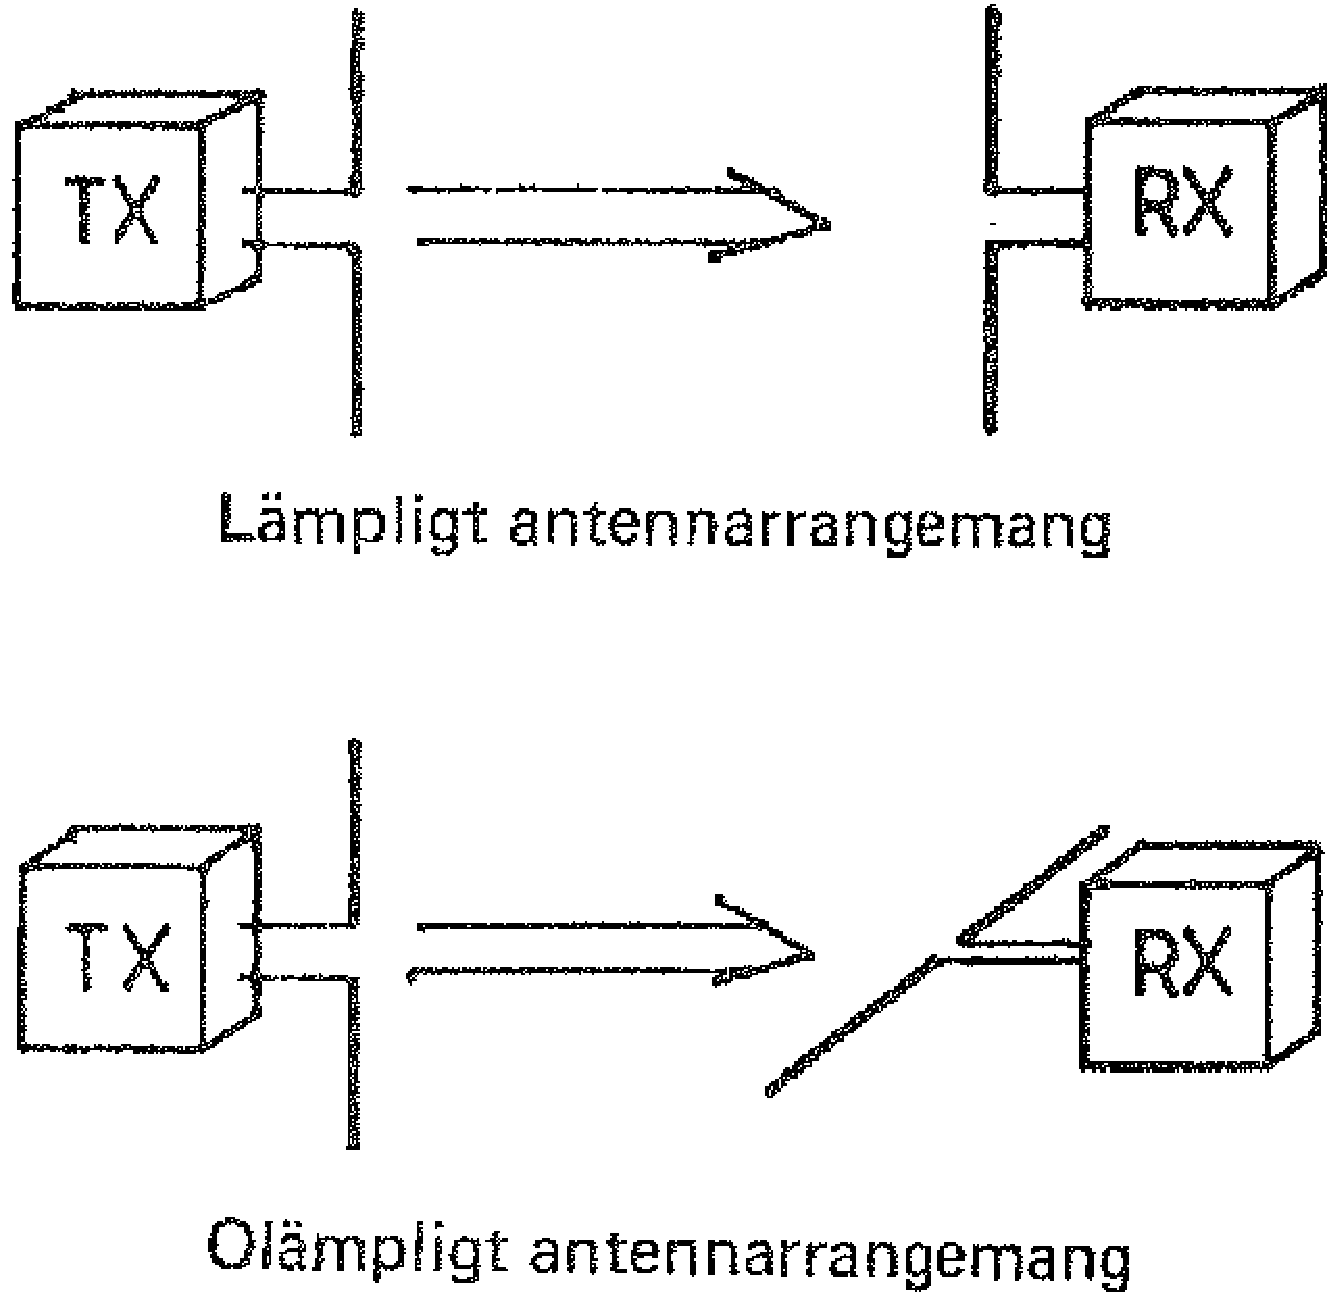
\includegraphics[width=0.5\textwidth]{images/cropped_pdfs/bild_2_6-11.pdf}
  \caption{Inverkan av polarisation}
  \label{fig:bildII6-11}
\end{wrapfigure}

I de högre frekvensområdena används både horisontell, vertikal eller
cirkulär polarisation.

Polarisationsriktningen ändras inte spontant under överföringen så
länge som vågorna inte reflekterats på vägen.
Vilken polarisation man väljer är av mindre betydelse än att den är lika
för både sändar- och mottagarantennen.

För cirkulärt polariserade antenner, där polarisationen vrider sig
omkring utbredningsaxeln, gäller att överföringen är bäst, när
vridningens riktning är lika både i sändar- och mottagarantennen.

Om en sändare som i det nedre delen av bild \ref{fig:bildII6-11} har vertikal
polarisation och mottagaren horisontell polarisation så dämpas den mottagna
signalstyrkan kraftigt.
Räknat i dB kan dämpningen i det olämpliga arrangemanget vara mer än 30~dB.
